% Indicate the main file. Must go at the beginning of the file.
% !TEX root = ../main.tex

%%%%%%%%%%%%%%%%%%%%%%%%%%%%%%%%%%%%%%%%%%%%%%%%%%%%%%%%%%%%%%%%%%%%%%%%%%%%%%%%
% 04_results
%%%%%%%%%%%%%%%%%%%%%%%%%%%%%%%%%%%%%%%%%%%%%%%%%%%%%%%%%%%%%%%%%%%%%%%%%%%%%%%%

\section{Results}
\label{results}

    \subsection{Detection}

    - after detection how many sequences are excluded

    - how many images are left per label

    \subsection{Classification Performance}

    All classification models performed well on their respective test sets.
    The balanced accuracy scores for each model are presented in \autoref{tab:bal_acc_by_model}.
    Generally, smaller models achieved slightly higher scores than larger ones, although these differences remained within one standard deviation.
    In particular, the pretrained EfficientNet-B0 reached the highest balanced accuracy of \(0.992\pm0.004\).
    Applying sequence level classification to the image level predictions improved balanced accuracy for every model, but only by \(0.001\) to \(0.005\), which again falls within a single standard deviation.

    Pretrained models consistently outperformed those trained from scratch, as shown in \autoref{fig:bal_acc_img}.
    EfficientNet-B0 with pretraining performs uniformly well across all folds, with only one outlier, while the non-pretrained version scored slightly lower on average and showed greater variability.
    In contrast the DenseNet-169 shows less of gap between pretrained and non-pretrained variants, with the pretrained variant performing slightly better but also increased spread across folds.
    ResNet-50 values were more dispersed for both variants, yet the pretrained model still held a clear advantage. 
    Finally, ViT-B/16 displayed the largest benefit from pretraining, alongside the greatest fold-to-fold variability in both its pretrained and non-pretrained versions.

    % table
    \begin{table}[H]
\centering
\caption{Balanced accuracy of all models -- shown as mean ± standard deviation.}
\label{tab:bal_acc_by_model}
\begin{tabular}{l c r c c}
\toprule
Model & Pretrained & Params (M) & Image BA-Score & Sequence BA-Score \\
\midrule
efficientnet\_b0 & Yes & 4 & 0.9921 ± 0.004 & 0.9947 ± 0.002 \\
densenet169 & Yes & 12 & 0.9904 ± 0.004 & 0.9939 ± 0.002 \\
resnet50 & Yes & 23 & 0.9899 ± 0.004 & 0.9934 ± 0.002 \\
vit\_b\_16 & Yes & 85 & 0.9885 ± 0.005 & 0.9933 ± 0.002 \\
\midrule
efficientnet\_b0 & No & 4 & 0.9856 ± 0.005 & 0.9898 ± 0.003 \\
densenet169 & No & 12 & 0.9863 ± 0.006 & 0.9899 ± 0.002 \\
resnet50 & No & 23 & 0.9850 ± 0.004 & 0.9888 ± 0.003 \\
vit\_b\_16 & No & 85 & 0.9767 ± 0.006 & 0.9856 ± 0.004 \\
\bottomrule
\end{tabular}
\end{table}

    \begin{figure}[ht]
    \centering
    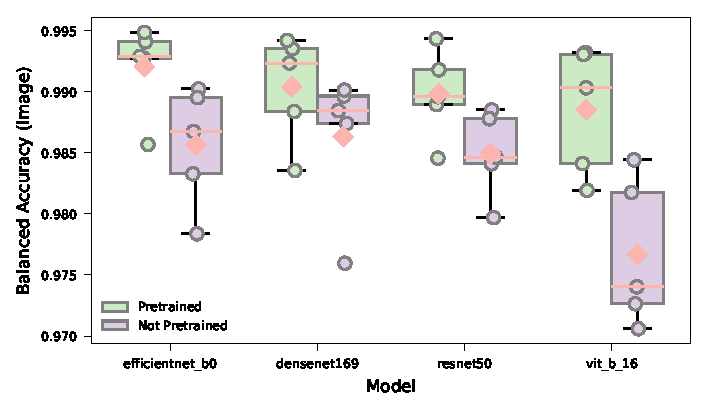
\includegraphics{figures/bal_acc_img.pdf}
    \caption{Balanced accuracy of each model on the image-level across folds, shown separately for pretrained and non-pretrained variants. Individual fold results are plotted as points; the mean balanced accuracy is marked by a diamond; and the median is indicated by a horizontal line.}
    \label{fig:bal_acc_img}
    \end{figure}

    \subsection{Best Model}

    The model with the best performance measured by balanced accuracy was the pretrained version of EfficientNet-B0.
    Its performance per category is shown in \autoref{tab:precision_recall_fscore_support}.
    The class it performed best on was \textit{mustela\_erminea} with a value of \(0.999\) for all metrics --- this happens to be one of the classes with with relatively little samples available.
    While it performed the worse on the other underrepresented class: \textit{soricidae} with a precision of \(0.971\), recall of \(0.979\) and F1-score of \(0.975\).
    For the other, more represented classes, the model achieved very high scores above \(0.99\) for all metrics.
    
    The Normalized Confusion Matrix for the best model is shown in \autoref{fig:conf_matrix_best}.
    It shows that there is basically no false positives for the class \textit{mustela\_erminea} while it was rarely confused for other classes.
    The most frequent misclassification occurred with \textit{soricidae} being falsely classified as \textit{apodemus\_sp} with a value of \(0.0184\).
    All other classes have a false positive rate of less than \(0.006\).

    % table
    \begin{table}[H]
\caption{Precision, recall and F1-score for the best model.}
\label{tab:precision_recall_fscore_support}
\begin{tabular}{l r r r r}
\toprule
Class & Precision & Recall & F1-Score & Support \\
\midrule
apodemus\_sp & 0.996 & 0.997 & 0.996 & 260075 \\
mustela\_erminea & 0.999 & 0.999 & 0.999 & 13175 \\
cricetidae & 0.995 & 0.993 & 0.994 & 144402 \\
soricidae & 0.971 & 0.979 & 0.975 & 12780 \\
\bottomrule
\end{tabular}
\end{table}


    \begin{figure}[ht]
    \centering
    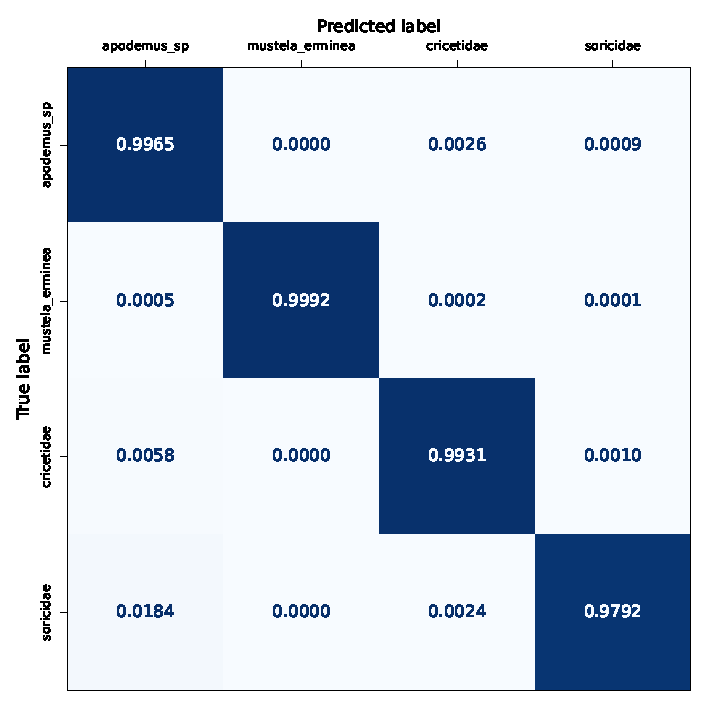
\includegraphics{figures/conf_matrix_best.pdf}
    \caption{Normalized Confusion Matrix for the best-performing model.}
    \label{fig:conf_matrix_best}
    \end{figure}
